%%%%%%%%% Packages %%%%%%%%%
\documentclass[aspectratio=169]{beamer}
\usepackage[T1]{fontenc}
\usepackage{pgfpages}

%%%%%%%%% Packages setup %%%%%%%%%
%\setbeameroption{show notes on second screen}
%\setbeameroption{show only notes}
%\setbeamerfont{note page}{size=\tiny}
\setbeamercolor{note page}{bg=white, fg=black}
\setbeamercolor{note title}{bg=white!99!black, fg=black}
%\usetheme{Hannover}
\usecolortheme{spruce}
\setbeamerfont{institute}{size=\scriptsize}
\graphicspath{{./figures/}{../figures/}}

%%%%%%%%% Document informations %%%%%%%%%
\title{Sensitivity analysis of climate change risk assessment}
\subtitle{Study of parameters variation in hazard indicators}
\author[Marco Casari]{%
  Marco Casari\\[2ex]%
  {\scriptsize Supervisors}\\%
  Prof.ssa Elisa Palazzi\\%
  Prof. Alberto Viglione\\%
}
\date[04/07/2024]{Midterm discussion, 4 July 2024}
\institute[UniTo]{University of Turin}

%%%%%%%%% Document %%%%%%%%%
\begin{document}
\begin{frame}
  \titlepage
\end{frame}



\section{Introduction}
\begin{frame}{Introduction}
  \begin{itemize}
    \item<1-> Risk: potential for adverse consequences for human or ecological systems [...]
    % 2021MatthewsAnnexVII
    \note[item]<1->{Few definitions to have a common starting point, all from IPCC AR6.}
    \item<2-> Climate Change Risk Assessment (CCRA)\\[1em]
    \begin{center}
      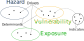
\includegraphics[keepaspectratio=true,width=0.5\textheight]{nomenclature}
    \end{center}
    \note[item]<2->{Estimation of risk related to climate change, i.e. determined by potential impacts of climate change and human responses to climate change.}
    % 2021MatthewsAnnexVII
    \note[item]<2->{Some additional definitions are needed, e.g. determinants of risk, risk drivers.}
    % 2021SimpsonAFramework
    \note[item]<2->{If quantitative, CCRA conveys numerical values combining the chosen indicators.}
  \end{itemize}
\end{frame}

\begin{frame}{The problem}
  \begin{itemize}
    \item<1-> The choice of indicators is arbitrary
    \note[item]<1->{Many methodologies and guidelines, different indicators may lead to different risks.}
    \item<2-> Analysis of the sensitivity of indicators to a change in value of their parameters, for drivers within the hazard determinant
  \end{itemize}
\end{frame}

\begin{frame}{Case study}
  \begin{itemize}
    \item<1-> Torino Airport
    % MC insert picture of geographical location, simple, box around Turin, with point on the coordinates and label with name of the city.
    \note[item]<1->{Exposure and vulnerability are fixed.}
    \item<2-> Hazard drivers: heat wave, heavy precipitation
    \note[item]<2->{Hazard drivers are from the European Taxonomy of climate hazards.}
    % 2024EU20212139
  \end{itemize}
\end{frame}



\section{Data}
\begin{frame}{Climate datasets}
  \begin{itemize}
    \item Climatological baseline: ERA5
    % 2018C3SERA5Hourly
    \item Climate projections: NEX-GDDP-CMIP6
    % NASAEarth
  \end{itemize}
  % MC maybe insert logo of the organizations, here or in the next slides on the datasets.
\end{frame}

\begin{frame}{ERA5}
  \begin{itemize}
    \item Organisation: European Centre for Medium-Range Weather Forecasts
    \item Data type: reanalysis
    \item Spatial resolution: 0.25° x 0.25°
    \item Time frequency: hour
  \end{itemize}
\end{frame}

\begin{frame}{NEX-GDDP-CMIP6}
  \begin{itemize}
    \item Organisation: NASA Earth Exchange
    \item Data type: statistically downscaled bias-corrected climate projections
    \item Spatial resolution: 0.25° x 0.25°
    \item Time frequency: day
    \item Historical period 1950-2014, projection period 2015-2100
    \item Model: EC-Earth3
    \note[item]{Only model EC-Earth3 is considered for the midterm discussion.}
    \item Scenario: SSP1-2.6, SSP2-4.5, SSP5-8.5
  \end{itemize}
\end{frame}

\begin{frame}{Spatial domain}
  \begin{itemize}
    \item Box of 3 x 3 grid points centred at the coordinates of the airport
  \end{itemize}
  % MC insert map as in frame Case study but with tiles of the variables for an example timestamp (e.g. anomaly in the same day of the presentation, for scenic effect).
\end{frame}

\begin{frame}{Temporal domain}
  \begin{itemize}
    \item Baseline period: 1994-2023
    \item Time horizons: 2021-2040, 2051-2070, 2081-2100
  \end{itemize}
  % MC put a pretty time line.
\end{frame}



\section{Methods}
% MC show with schemes and matrices the idea of varying the hazard indicators and study the statistics of the resulting ensembles.

\begin{frame}{Methodology}
  \begin{itemize}
    \item<1-> Indicators: heat wave frequency, maximum $n$-days precipitation
    \note[item]<1->{The $n$ is one of the parameters of the indicator. Select intervals of variation of parameters and evaluate indicators for each combination of them.}
    \item<1-> Fixed exposure and vulnerability from literature
    \item<2-> Evaluate risk following the guidelines
    \note[item]<2->{A value for each determinant is evaluated, which is the aggregation of the respective indicators. The aggregation include also a normalisation step, hence the final value is in the interval $[0, 1]$ and values from different determinants can be compared to each other. Risk is the weighted mean of those values and in this project the weights are set to 1 because exposure and vulnerability are constant, hence the relation between risk and hazard is linear and no interesting information is added by considering different weigths. Finally the risk values are classified in a rank of 5 classes, by splitting the interval $[0, 1]$ in 5 equally sized subintervals.}
    % MC add formula for risk.
    % 2017GIZRiskSupplement
  \end{itemize}
\end{frame}

% MC add frame Indicators which shows the definitions of the chosen indicators. Remove from the final discussion because it takes too long.

% \begin{frame}{Preprocessing}
%   \begin{enumerate}
%     \item<1-> Regrid ERA5
%     \note[item]<1->{Since resolution is the same, a simple traslation of coordinates is sufficient. Use convention of NEX-GDDP-CMIP6: coordinates are the centre of the grid points.}
%     \item<2-> Aggregate ERA5 at daily frequency
%     \note[item]<2->{Total precipitation is summed, other quantities are averaged.}
%     \item<3-> Align NEX-GDDP-CMIP6 timestamps
%     \note[item]<3->{At daily resolution timestamps differ by hours of the same day, the offset loses meaning when aggregation at daily frequency is applied. Use convention of ERA5: timestamps point to the start of the day.}
%     \item<4-> Bias adjustment\\[0.5em]
%     \begin{center}
%       \begin{minipage}{0.6\linewidth}
%         \centering
%         \begin{tabular}{ccc}
%           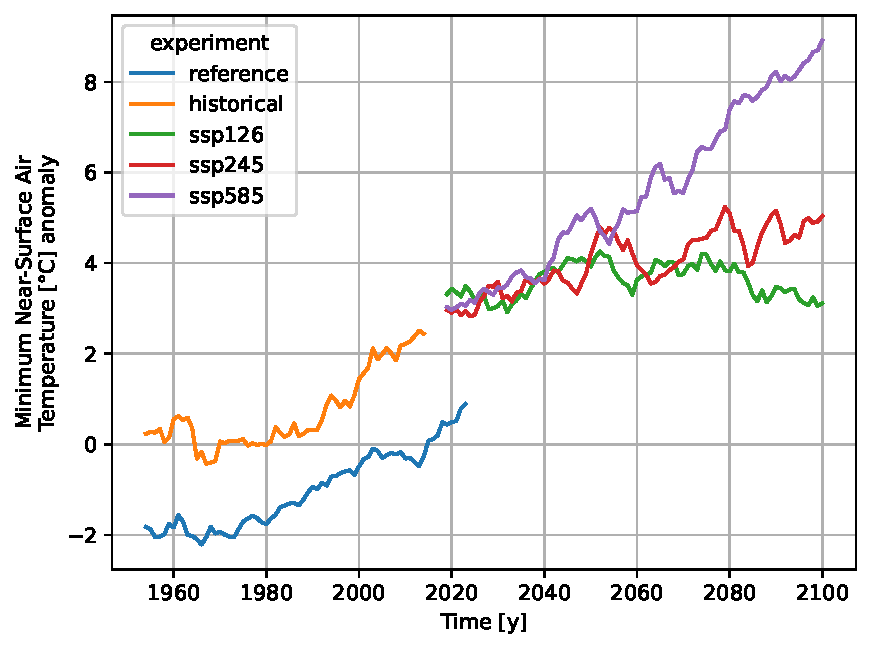
\includegraphics[width=0.30\linewidth]{tasmin_anomaly_preprocessed} & 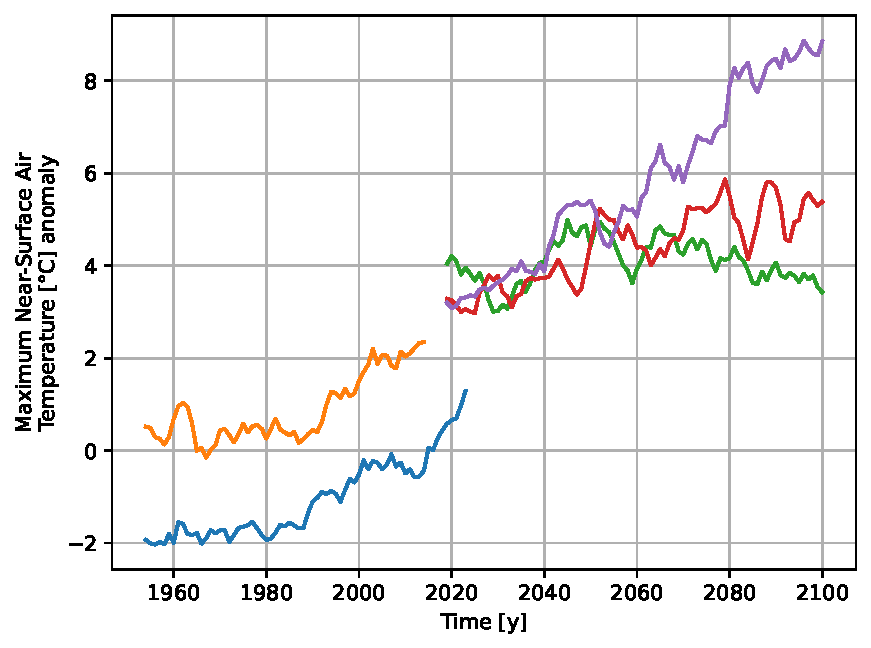
\includegraphics[width=0.30\linewidth]{tasmax_anomaly_preprocessed} & 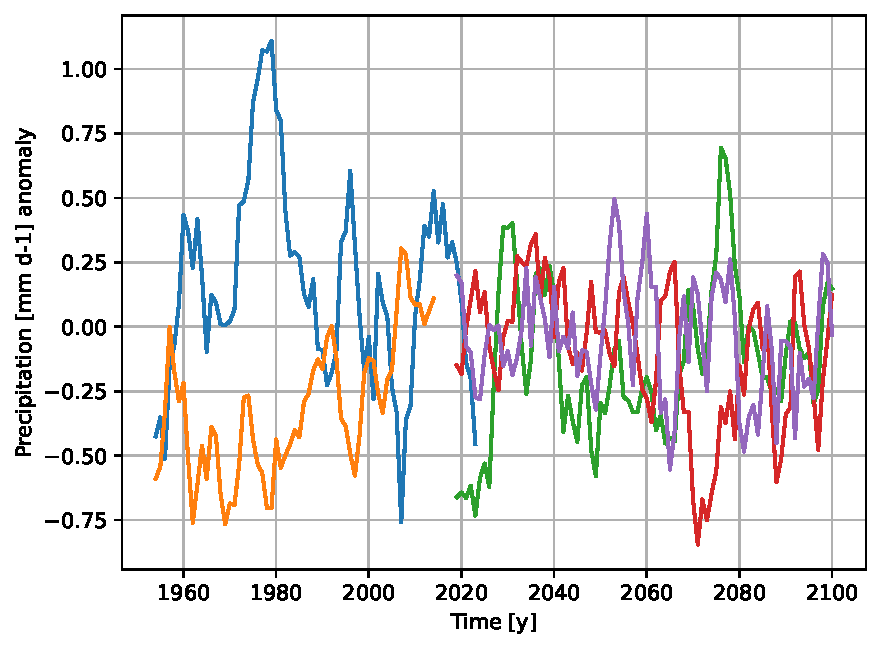
\includegraphics[width=0.30\linewidth]{pr_anomaly_preprocessed} \\
%           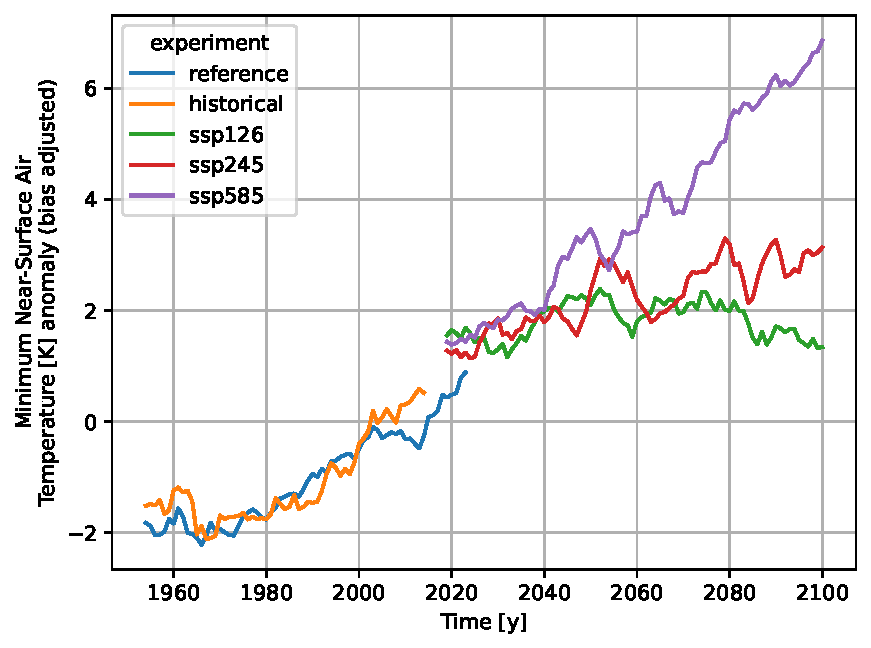
\includegraphics[width=0.30\linewidth]{tasmin_anomaly_adjusted} & 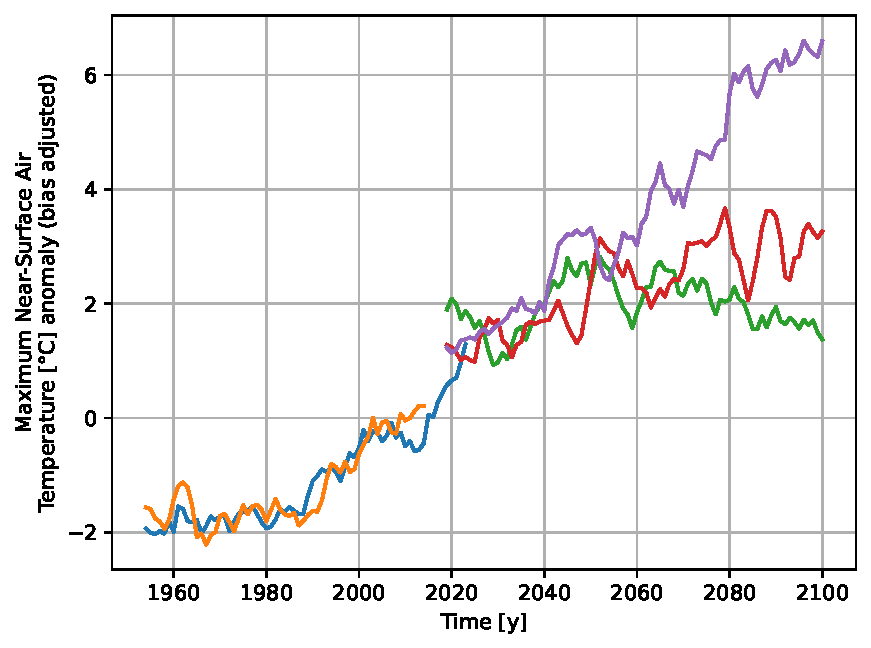
\includegraphics[width=0.30\linewidth]{tasmax_anomaly_adjusted} & 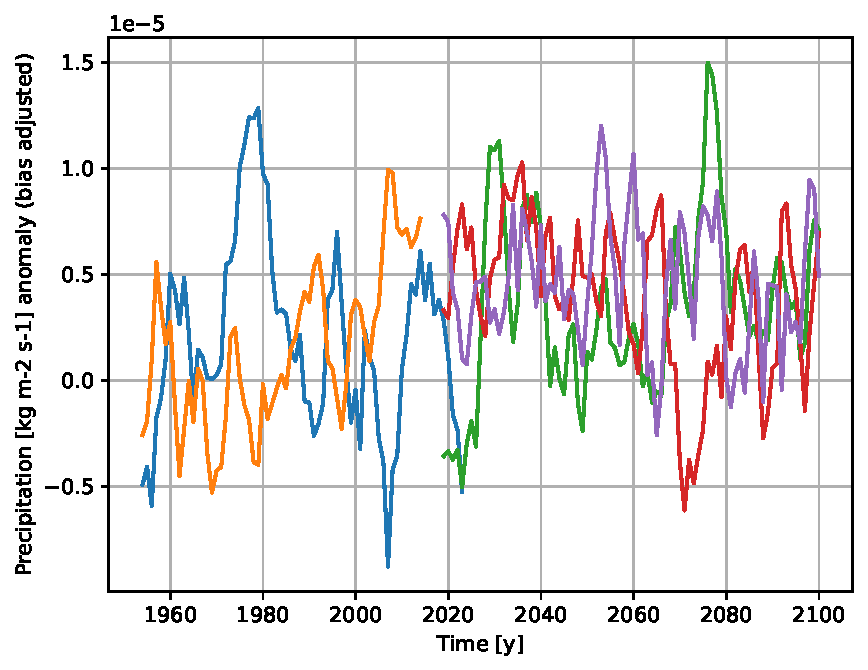
\includegraphics[width=0.30\linewidth]{pr_anomaly_adjusted}
%         \end{tabular}
%       \end{minipage}\hfill
%       \begin{minipage}{0.3\linewidth}
%         \centering
%         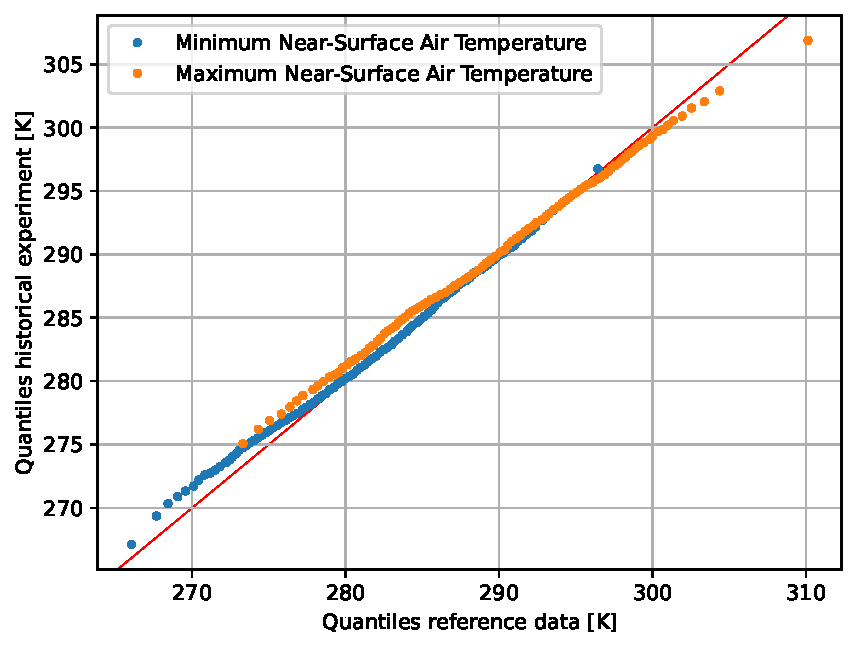
\includegraphics[width=0.5\textheight]{temperature_q-q_plot}\\
%         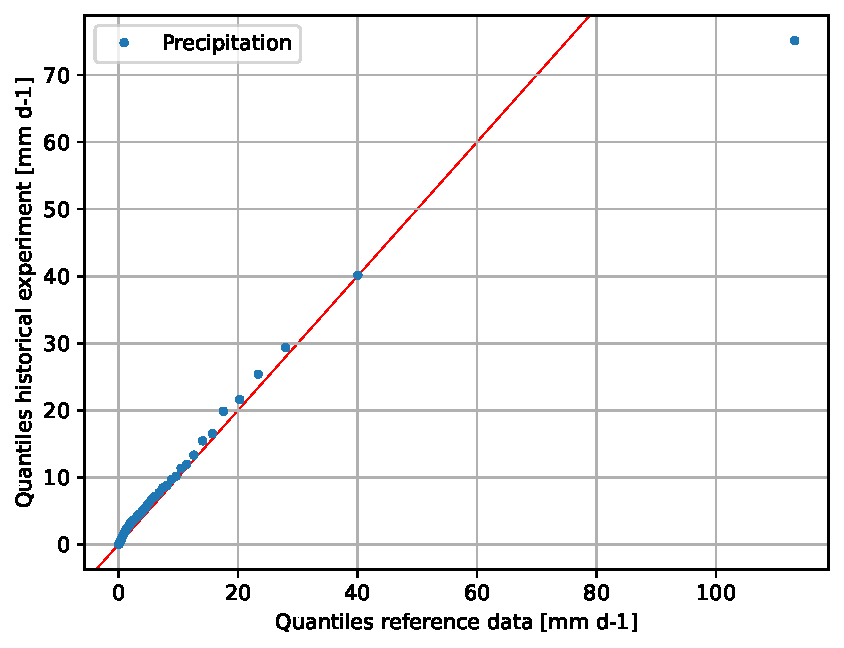
\includegraphics[width=0.5\textheight]{precipitation_q-q_plot}
%       \end{minipage}
%     \end{center}
%     \note[item]<4->{Training period 1950-1999, test period 2000-2014. Additive Quantile Delta Mapping for both temperature and precipitation, show p-p plot for qualitative assessment of the adjustment. THe figures refere to the coordinates of grid point containing the airport.}
%     % MC extend historical period to 2023 with one period from the projections?
%   \end{enumerate}
% \end{frame}

\begin{frame}{Preprocessing}
\begin{columns}[T]
\begin{column}{0.60\textwidth}
  \begin{enumerate}
    \item<1-> Regrid ERA5
    \note[item]<1->{Since resolution is the same, a simple traslation of coordinates is sufficient. Use convention of NEX-GDDP-CMIP6: coordinates are the centre of the grid points.}
    \item<1-> Aggregate ERA5 at daily frequency
    \note[item]<1->{Total precipitation is summed, other quantities are averaged.}
    \item<1-> Align NEX-GDDP-CMIP6 timestamps
    \note[item]<1->{At daily resolution timestamps differ by hours of the same day, the offset loses meaning when aggregation at daily frequency is applied. Use convention of ERA5: timestamps point to the start of the day.}
    \item<2-> Bias adjustment
    \note[item]<2->{Training period 1950-1999, test period 2000-2014. Additive Quantile Delta Mapping for both temperature and precipitation, show p-p plot for qualitative assessment of the adjustment. THe figures refere to the coordinates of grid point containing the airport.}
    % MC extend historical period to 2023 with one period from the projections?
  \end{enumerate}
  \visible<2->{
  \begin{center}
    \begin{tabular}{ccc}
      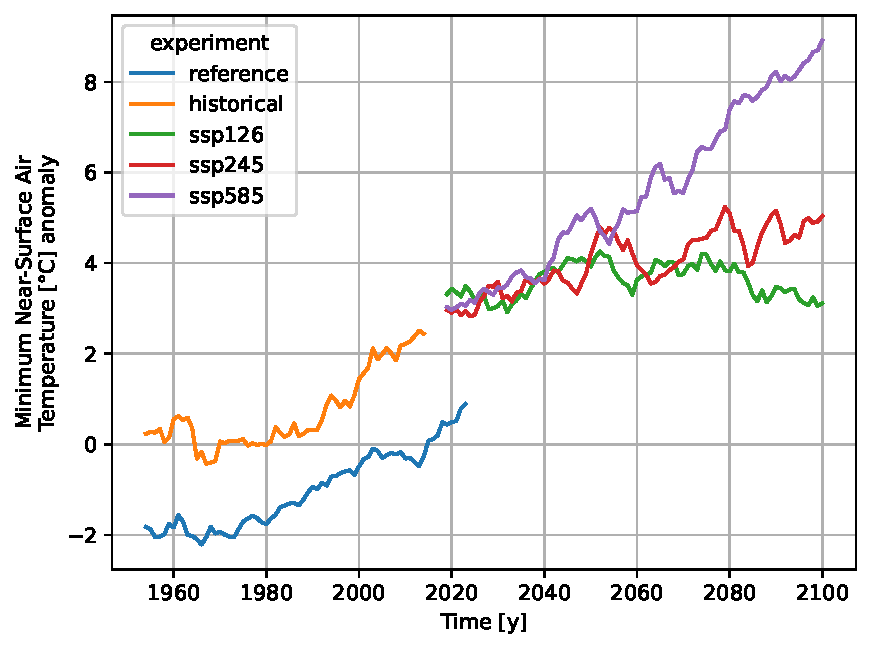
\includegraphics[width=0.25\columnwidth]{tasmin_anomaly_preprocessed} & 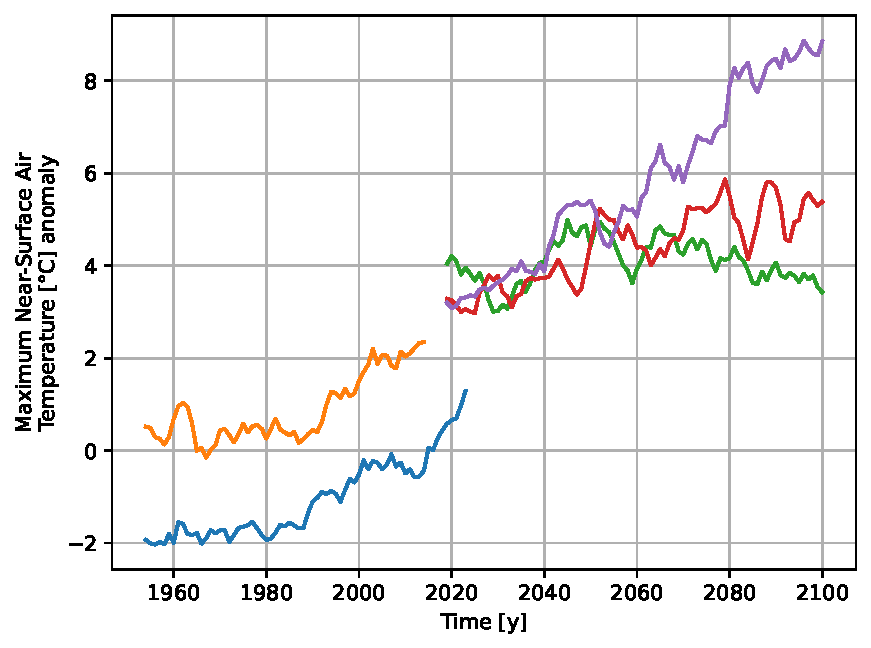
\includegraphics[width=0.25\columnwidth]{tasmax_anomaly_preprocessed} & 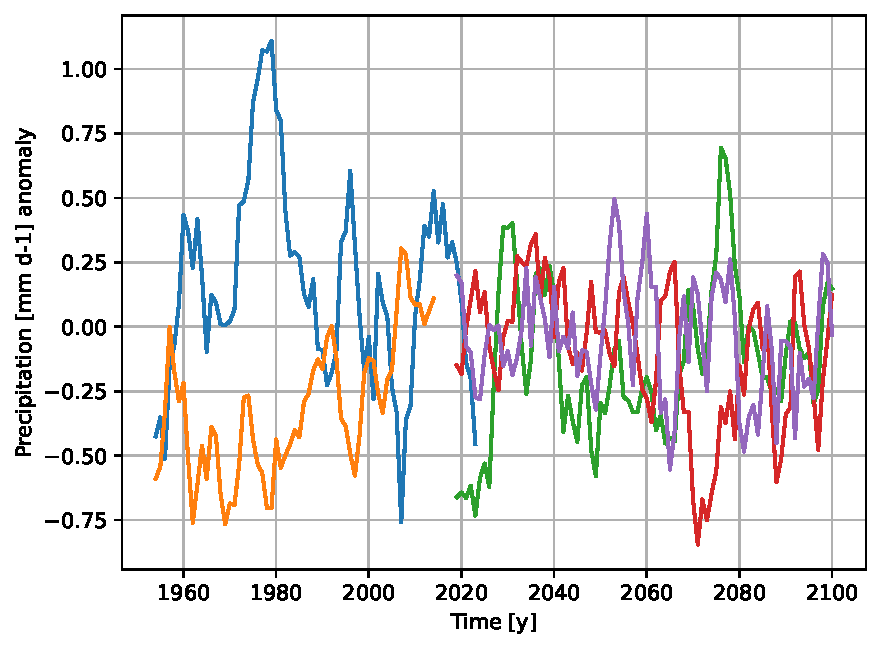
\includegraphics[width=0.25\columnwidth]{pr_anomaly_preprocessed} \\
      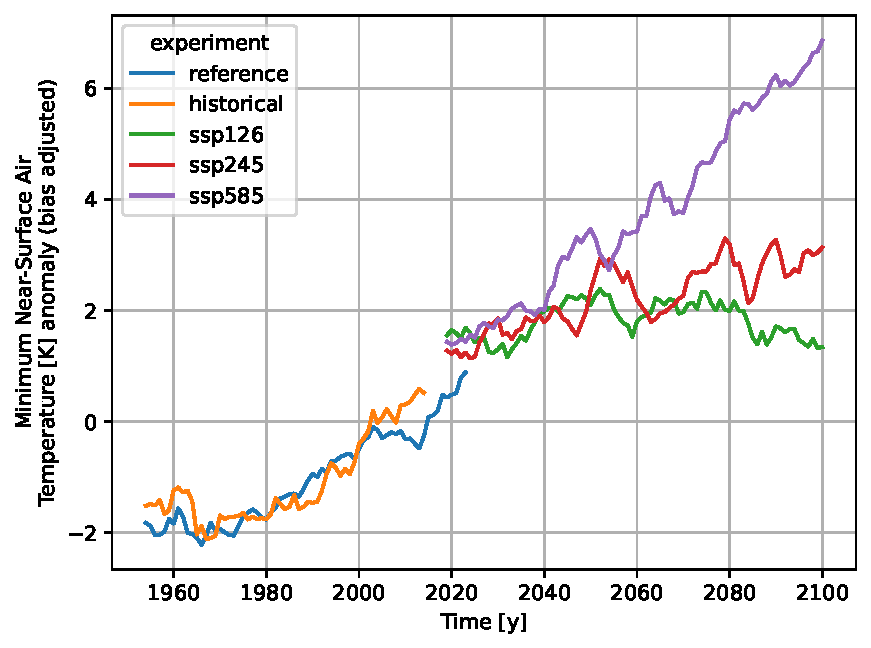
\includegraphics[width=0.25\columnwidth]{tasmin_anomaly_adjusted} & 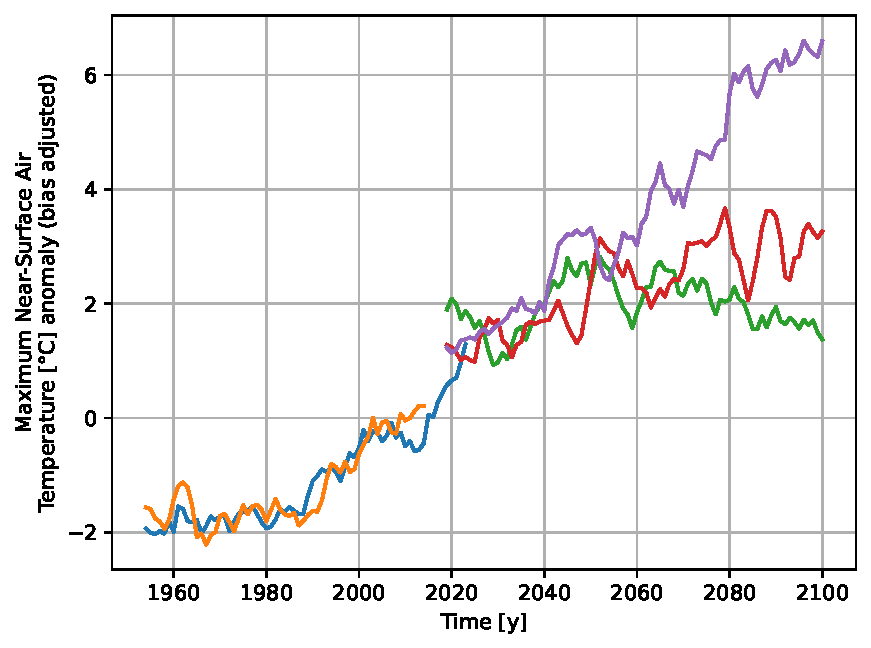
\includegraphics[width=0.25\columnwidth]{tasmax_anomaly_adjusted} & 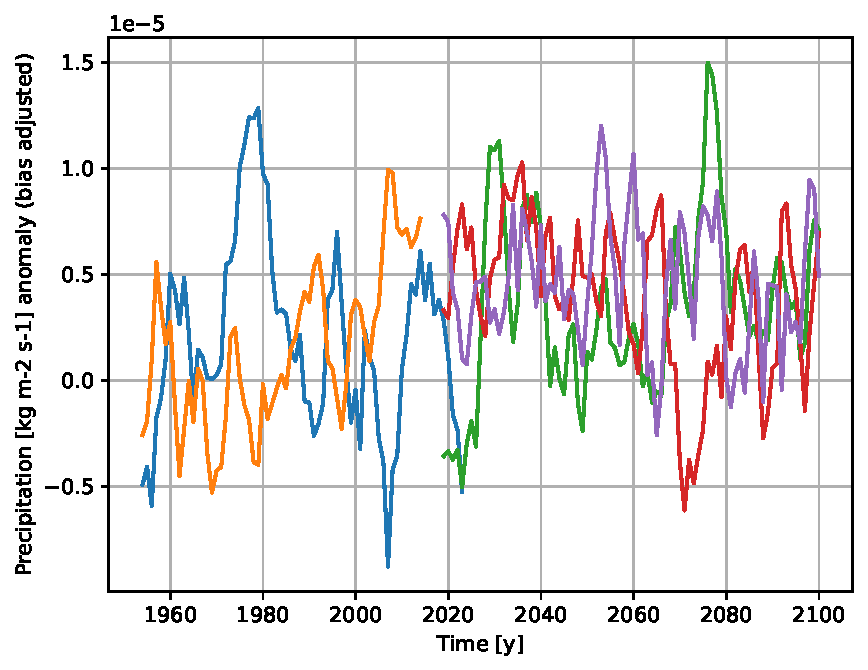
\includegraphics[width=0.25\columnwidth]{pr_anomaly_adjusted}
    \end{tabular}
  \end{center}
  }
\end{column}
\begin{column}{0.40\textwidth}
  \visible<3->{
  \begin{center}
    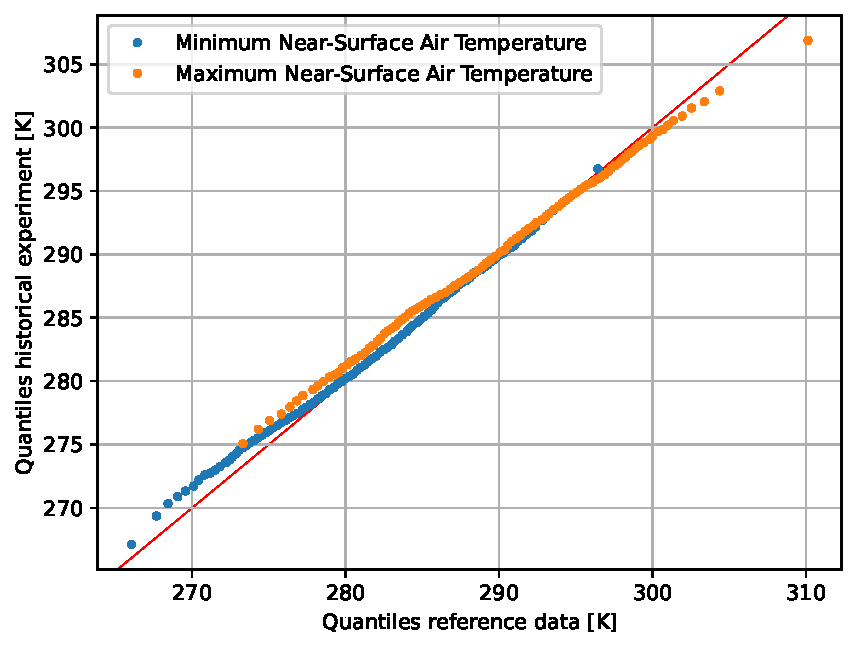
\includegraphics[width=0.47\textheight]{temperature_q-q_plot}\\
    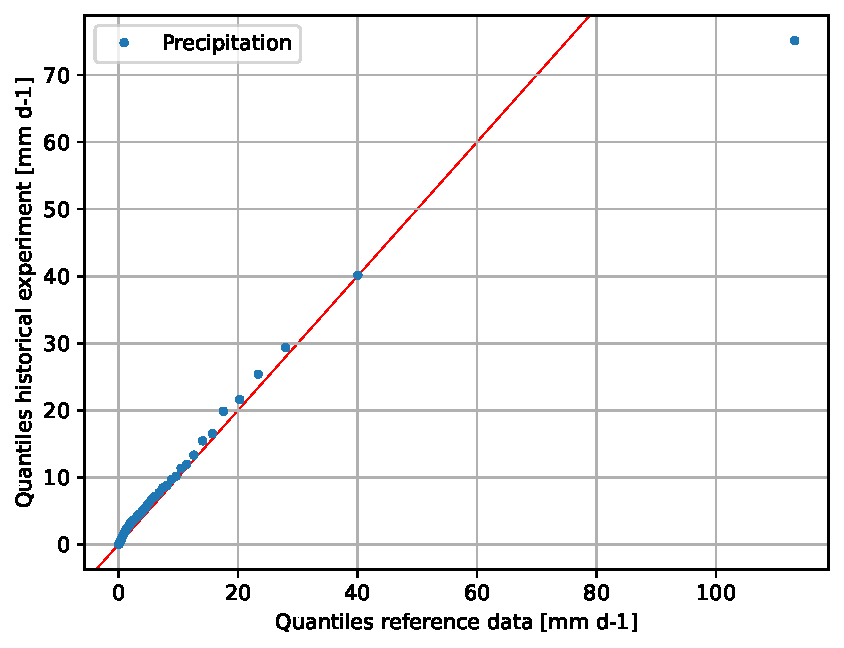
\includegraphics[width=0.47\textheight]{precipitation_q-q_plot}
  \end{center}
  }
\end{column}
\end{columns}
\end{frame}
% MC rearrange figures to make them more readable.

\begin{frame}{Evaluation of hazard indicators}
\begin{columns}[c]
\begin{column}{0.60\textwidth}
  \begin{enumerate}
    \item<1-> Define intervals of parameter values
    \note[item]<1->{Less dense for regions of slowly varying quantile function.}
    \item<2-> Spatial aggregation
    \note[item]<2->{Sample average, check standard deviation.}
    % MC try EOF?
    \item<3-> Temporal aggregation
    \note[item]<3->{Sample average, check standard deviation.}
    % MC try Mann-Kendall, check compatiblity of Senn slope with 0?
    \item<4-> Risk evaluation
    \note[item]<4->{Given exposure and vulnerability, evaluate the final risk.}
  \end{enumerate}
\end{column}
\begin{column}{0.40\textwidth}
  \visible<1>{
  \begin{center}
    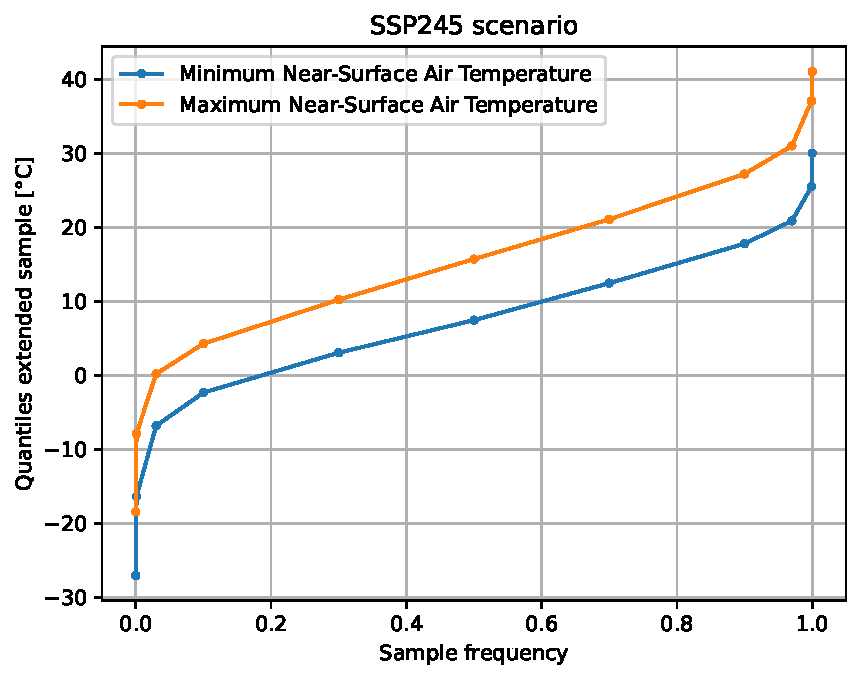
\includegraphics[width=0.47\textheight]{temperature_quantile_ssp245_sample}\\
    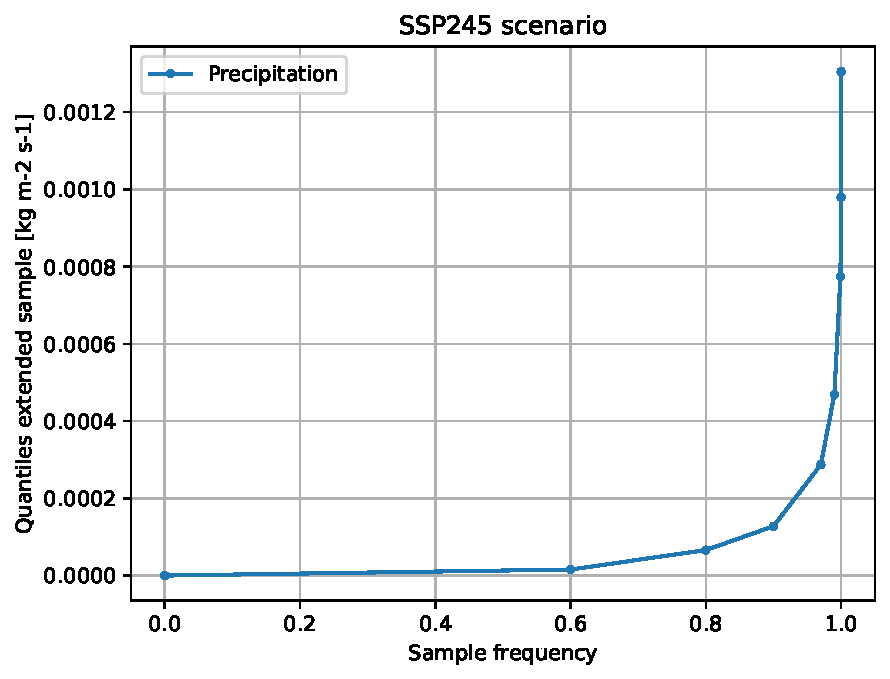
\includegraphics[width=0.47\textheight]{precipitation_quantile_ssp245_sample}
  \end{center}
  }
\end{column}
\end{columns}
\end{frame}

%\section{Case study}
% MC talk about airports, the hazard drivers affecting them and the chosen indicators.

\section{Results and discussion}
\begin{frame}{Heat wave frequency}
  % MC show plot of hazard for range thresh_tasmax [288.7, 309.1].
\end{frame}

%\section{Conclusion}
% MC resume the initial idea and how the results obtained at this point match it.
% MC list some criticalities I am having at this point.

\begin{frame}{Next steps}
  \begin{itemize}
    \item Uncertainty evaluation
    \item Evaluate risk with non-linear relations among hazard indicators and among determinants
    \item Extend analysis to Bologna's and Ciampino's airports
    \item Choose points of the interval more appropriate for the location of interest
  \end{itemize}
\end{frame}

\end{document}
